\documentclass[a4paper]{article}

\usepackage[french]{babel}
\usepackage[T1]{fontenc}
\usepackage[utf8]{inputenc}
\usepackage{amsmath}
\usepackage{graphicx}
\usepackage{lmodern}
\usepackage[left=3cm, right=3cm, bottom=4cm, top=4cm]{geometry}
\usepackage{array}
\usepackage{pdfpages}
\usepackage{listings}
\usepackage{algorithm}
\usepackage{algorithmic}
\usepackage{sidecap}
\usepackage{pdflscape}
\usepackage{hyperref}
\usepackage{tipa}
\usepackage{multirow}
\usepackage[gen]{eurosym}
\DeclareUnicodeCharacter{20AC}{\euro{}}

\usepackage{hyperref}
\hypersetup{    
    colorlinks,
    citecolor=black,
    filecolor=black,
    linkcolor=black,
    urlcolor=black
}

\title{Rapport de planification}

\author
{
    Pierre-Marie {\sc Airiau}\\
    Valentin {\sc Esmieu}\\
    Hoel {\sc Kervadec}\\
    Maud {\sc Leray}\\
    Florent {\sc Mallard}\\
    Corentin {\sc Nicole}
}

\date{\today}

\newcommand{\pagevierge}[0]{\newpage\thispagestyle{empty}\null\newpage}
\newcommand{\glasir}[0]{Glasir}
\newcommand{\ttable}[0]{{\sc Table}}
\newcommand{\ffigure}[0]{{\sc Figure}}

\newcommand{\nomRepart}[1]{\multicolumn{2}{c||}{\textbf{#1}}}
\newcommand{\nomRepartt}[1]{\multicolumn{2}{c|}{\textbf{#1}}}

\begin{document}
    % Ouh c'est sale.
    \hypersetup{pageanchor=false}
    
\includepdf[pages=1]{figure/couv.pdf}
    \hypersetup{pageanchor=true}
    
    \newpage
    \thispagestyle{empty}
    \mbox{}
    
    \newpage
    % A decommenter pour la release
    % \setcounter{tocdepth}{2}
    \tableofcontents
    \setlength{\parskip}{10pt}
    
    \newpage
    \thispagestyle{empty}
    \mbox{}

    \newpage
    \section{Introduction}
	La sécurisation des systèmes est une problématique majeure de la société moderne. En ce sens, de nombreuses méthodologies ont été développées~\cite{introSecurite,ADTreeKordy} dans le but d'identifier les risques et de les quantifier. C'est avec cet objectif que le concept d'arbres d'attaque et de défense (ADTrees) a vu le jour.

	Lors de la phase de pré-étude, nous avons pu comprendre l’intérêt pratique de la construction des ADTrees. Leur utilisation permet d'identifier de manière précise les différentes attaques possibles contre un système et de les valuer en termes de coût, de probabilité, etc. ADTool~\cite{adtool_paper} (Attack-Defense Tree Tool), un logiciel libre développé pour l'implémentation de ces arbres sur support informatique, a été mis à disposition pour ce projet. Lors de sa prise en main, des limites ont été constatées. En effet, dans un cas concret d'expertise en sécurité, le système doit faire face à une multitude d'attaques possibles et, par conséquent, l'ADTree qui les modélisera sera de très grande taille. Dans ce cas, il est très difficile pour l'expert d'en extraire des informations pertinentes au premier coup d’œil. Or, ADTool ne fournit pas d'outil permettant à l'utilisateur de simplifier l'analyse de l'arbre. 

	L'objectif de ce projet est donc la création d'un logiciel intégrant ADTool et permettant de faciliter le travail d'un expert en sécurité, en lui fournissant des outils pour analyser facilement ses ADTrees. Ce logiciel portera le nom de \glasir{}  (prononcé [\textipa{glaziK}]). Il s'agit du nom d'un arbre aux feuilles d'or dans la mythologie nordique~\cite{vikingCulture}.

	Ce rapport présente les spécifications fonctionnelles de \glasir{}. Tout d'abord, les limites d'ADTool seront abordées, afin de justifier l'intérêt de \glasir{}. Puis nous détaillerons les différentes fonctionnalités destinées à l'analyse des ADTrees. Enfin, quelques améliorations supplémentaires seront également précisées pour offrir un meilleur confort de création et édition d'arbres. Ces spécifications seront faites en prenant en exemple une situation précise : celle d'un expert en sécurité chargé par le Service des Transports en commun de l'Agglomération Rennaise (STAR) de déterminer les failles de leurs systèmes de paiement.

    \newpage
    \section{Contexte}
	\label{sec:retrospective}
	
\subsection{Périmètre fonctionnel}

\subsection{Éléments en entrée}

\subsection{Rétrospective}
	\label{sec:retrospective}

	Nous avons déjà rédigé deux rapports dans le cadre de ce projet, nous permettant d'en aborder différents aspects. Leur contenu est brièvement rappelé ci-dessous.

	\paragraph{Rapport de pré-étude} Nous avons commencé ce projet par une étude de l'existant : la théorie des ADTrees ainsi que la découverte d'ADTool, un logiciel permettant d'en créer et d'en manipuler. Nous avons relevé lors de cette étude des lacunes empêchant une analyse poussée des ADTrees. Le contexte (transports en commun, plus particulièrement le STAR) a lui aussi été traité, afin de mieux cerner notre cas d'étude. Il est apparu que les attaques contre les transports en commun sont assez fréquentes, qu'elles soient volontaires ou non. Nous entendons par \og attaque \fg{} tout événement nuisant au bon fonctionnement du réseau de transport. Suite à cela, nous avons été en mesure de proposer un premier cahier des charges. Ce dernier a été étoffé et précisé dans le second rapport.

	\paragraph{Rapport de spécifications fonctionnelles} Les fonctionnalités du logiciel ont été décrites de façon exhaustive. Cela nous a permis de fournir une première ébauche de l'architecture de \glasir{}, comprenant les dépendances entre les modules, et d'établir les différents liens les unissant. Cela nous a donné une vision plus globale et claire du projet, nous permettant de hiérarchiser les tâches à effectuer. Pour finir, nous avons proposé une planification succincte, développée dans le présent rapport. Celle-ci prévoyait la séparation du développement en de nombreuses versions.

	Celles-ci ont évolué depuis, et sont présentées en détail dans la section suivante.
    
    \section{Méthode de gestion de projet}
	\label{sec:gestion}


Au cours de nos réunions, nous nous sommes naturellement dirigés vers une méthode agile ressemblant à \og Scrum \fg. Nous nous réunissons une fois par semaine afin de discuter de l'avancement de nos tâches respectives et faire part de nos difficultés. Nous définissons en fonction de cela des tâches à effectuer la semaine suivante. 
	Chaque version sera composée de sprints au cours desquels nous nous consacrerons à un sous-ensemble de tâches nécessaires à une version. %whattt ???
	

		
    \section{Tâches unitaires}
	\label{sec:taches_unitaires}

	Les tests unitaires étants réalisés au fûr et à mesure, ils sont prit en compte dans l'estimation du temps nécessaire à la réalisation des tâches.

	\subsection{Version intermédiaire 1}

		\begin{table}[h]
			\centering
			\begin{tabular}{|c|r|l|c|r|}
				\hline
				\textbf{Cible} & \textbf{Id} & \textbf{Tâche} & \textbf{Technologies} & \textbf{Durée}\\
				\hline

				\multirow{5}{*}{\glasir{}} & 1.1 & Créer squelette interface & WPF & 3h\\
				\cline{2-5}
				 & 1.2 & Gestion des fichiers du projet & C\# & 10h\\
				\cline{2-5}
				 & 1.3 & Intégrer ADTool dans application & JNI & 10h\\
				\cline{2-5}
				 & 1.4 & \'Evaluateur de fonction & Java & 6h\\
				\cline{2-5}
				 & 1.5 & Interface évaluateur & WPF & 4h\\
				\hline

				\multirow{3}{*}{ADTool} & 1.6 & Valuer arbre & \multirow{3}{*}{Java} & 9h\\
				\cline{2-3} \cline{5-5}
				 & 1.7 & Refonte du langage des arbres & & 8h\\
				\cline{2-3} \cline{5-5}
				 & 1.8 & Vue globale des paramètres & & 6h\\
				\hline

				\multicolumn{4}{|l|}{\bf Total} & {\bf 56h}\\
				\hline
			\end{tabular}
			\caption{Tableau tâches version intermédiaire 1}
			\label{fig:taches_units_1}
		\end{table}

	\subsection{Version intermédiaire 2}

		\begin{table}[h]
			\centering
			\begin{tabular}{|c|r|l|c|r|}
				\hline
				\textbf{Cible} & \textbf{Id} & \textbf{Tâche} & \textbf{Technologies} & \textbf{Durée}\\
				\hline

				\multirow{4}{*}{\glasir{}} & 2.1 & Algorithme de filtrage & C++ & 24h\\
				\cline{2-5}
				 & 2.2 & Interface filtre & WPF & 15h\\
				\cline{2-5}
				 & 2.3 & Multiples instances d'ADTool & C++, WPF & 15h\\
				\cline{2-5}
				 & 2.4 & Affichage de l'arbre filtré & C++, WPF & 5h\\
				\hline

				\multirow{1}{*}{ADTool} & 2.5 & Couper/copier/coller & \multirow{1}{*}{Java} & 10h\\
				\hline

				\multicolumn{4}{|l|}{\bf Total} & {\bf 69h}\\
				\hline
			\end{tabular}
			\caption{Tableau tâches version intermédiaire 2}
			\label{fig:taches_units_2}
		\end{table}

	\subsection{Version finale}

		\begin{table}[h]
			\centering
			\begin{tabular}{|c|r|l|c|r|}
				\hline
				\textbf{Cible} & \textbf{Id} & \textbf{Tâche} & \textbf{Technologies} & \textbf{Durée}\\
				\hline

				\multirow{4}{*}{\glasir{}} & 3.1 & Optimiseur & C++, WPF & 15h\\
				\cline{2-5}
				 & 3.2 & Bibliothèque de modèles & C++, WPF & 10h\\
				\cline{2-5}
				 & 3.3 & Harmonisation interface & WPF & 5h\\
				\cline{2-5}
				 & 3.4 & Packaging & ? & 10h\\
				\hline

				\multirow{1}{*}{ADTool} & 3.5 & Ctrl-z & \multirow{1}{*}{Java} & 8h\\
				\hline

				\multicolumn{4}{|l|}{\bf Total} & {\bf 48h}\\
				\hline
			\end{tabular}
			\caption{Tableau tâches version finale}
			\label{fig:taches_units_3}
		\end{table}    
		
    %\section{Organisation}
	\label{sec:livrables}

	Au cours de nos réunions, nous nous sommes naturellement dirigés vers une méthode agile ressemblant à \og Scrum \fg. Nous nous réunissons une fois par semaine afin de discuter de l'avancement de nos tâches respectives et faire part de nos difficultés. Nous définissons en fonction de cela des tâches à effectuer la semaine suivante. Ainsi, nous avons décidé de livrer trois versions de \glasir{}, dont 2 intermédiaires.
	Chaque version sera composée de sprints au cours desquels nous nous consacrerons à une partie des tâches composant une version.
	Nous présentons ci-dessous la répartition des livrables :
	
	\begin{itemize}
		\item{v 0.1} Paramètres de synthèse :
		\begin{itemize}
			\item{sprint 1} Implémenter l'IHM, y intégrer ADTool, créer un projet, l'afficher dans l'arborescence ;
			\item{sprint 2} Évaluer une formule dans ADTool, la propager dans l'arbre, améliorer le codage des arbres ;
			\item{sprint 3} Rendre visibles plusieurs paramètres, communiquer les formules entre ADTool et \glasir{}, documenter le code et tester ;
		\end{itemize}
		\item{v 0.2} filtre :
		\begin{itemize}
			\item{sprint 1} Définir l'algorithme de filtrage, créer l'IHM ;
			\item{sprint 2} Créer un panneau dans \glasir{}, afficher l'arbre résultat, tester ;
			\item{sprint 3} Documenter le code, ouverture simultanée de plusieurs arbres ;
		\end{itemize}
		\item{v 1.0} optimiseur :
		\begin{itemize}
			\item{sprint 1} Implémenter l'algorithme de calcul du chemin optimal, créer le panneau associé dans l'IHM ;
			\item{sprint 2} Annuler une action, créer une bibliothèque de modèles, créer la page HTML ;
			\item{sprint 3} Documenter le code, harmoniser les graphismes.
		\end{itemize}
	\end{itemize}


	Ce plan d'action est amené à changer au fur et à mesure de sa réalisation, ces évolutions étant le but même des méthodes dites \og agiles \fg.
	
	\paragraph{Version intermédiaire 1}


	\paragraph{Version intermédiaire 2}

	\paragraph{Version finale}


    \section{Risques}
    Nous pouvons d'ores et déjà envisager des situations dans lesquelles nous ne serions pas en mesure de livrer le projet dans l'état que nous avions prévu en ce début d'année scolaire.
    Le facteur principal est bien entendu humain. En effet, la moitié du groupe partant étudier à l'étranger dans le cadre de la mobilité internationale, il se peut que nous ayons légèrement sur-estimé nos capacités de travail et annoncé une tâche trop difficile à exécuter. De plus, sur les trois personnes restant en France, une incapacité à travailler sur le projet, quelle qu'elle soit, aurait des répercussions sur l'avancée globale du livrable. Mais une incapacité de ce type serait accidentelle et très peu probable.
    
    Des problèmes d'ordre technique peuvent également survenir. Il est ainsi possible que nous rencontrions des difficultés à mettre en place la chaîne logicielle prévue, la plupart d'entre nous n'en ayant jamais développé. Nous pourrions ainsi connaître des problèmes dans la communication des différents composants de la chaîne logicielle. Il faudra, pour éviter cela, bien choisir les langages utilisés dans la conception logicielle.
    Une perte de données stockées sur Git, ou bien de fauses manipulations entrainant une perte de données totale ou partielle ralentirait \textit{a minima} le projet, et dans le pire des cas le rendrait impossible à livrer tel que nous l'avons promis. Cependant, Git est équipé d'outils de récupération pour les \textit{commit}, et le projet sera normalement mis à jour (\textit{pull}) sur chacun de nos ordinateurs personnels, réduisant quasimment ce risque à zéro.


    \section{Répartition}
	\label{sec:repartition}

	PM fera tous les tests parce qu'il est trop fort.

    \section{Séquencement}
	\label{sec:sequencement}
	Pour établir notre planification, nous avons utilisé le logiciel MS Project. Les diagrammes ci-dessous tiennent compte des différents jalons qui ont été posés, soit imposés à tous dans les projets de 4INFO, soit définis nous-même.

	\subsection{Diagramme de Gantt}
		Le diagramme de Gantt visible sur la \ffigure{} \ref{fig:gantt} illustre le séquencement de notre projet. Les tâches ont été attribuées à une personne, et les durées ont été calculées pour une moyenne d'une heure-et-demi de travail personnel par jour. Les semaines du 18 et 25 mai, bloquées pour les 4INFO, la durée du travail personnel a été porté à 4h par jour. 

	\subsection{Répartition de la charge de travail}
		Le planning de la \ffigure{} \ref{fig:planning_charge} illustre le cumul des heures de travail pour chaque personne. Nous avons essayé d'être homogènes dans la répartition des tâches de chacun.

		\begin{landscape}
		 	\begin{figure}
	            \centering
	            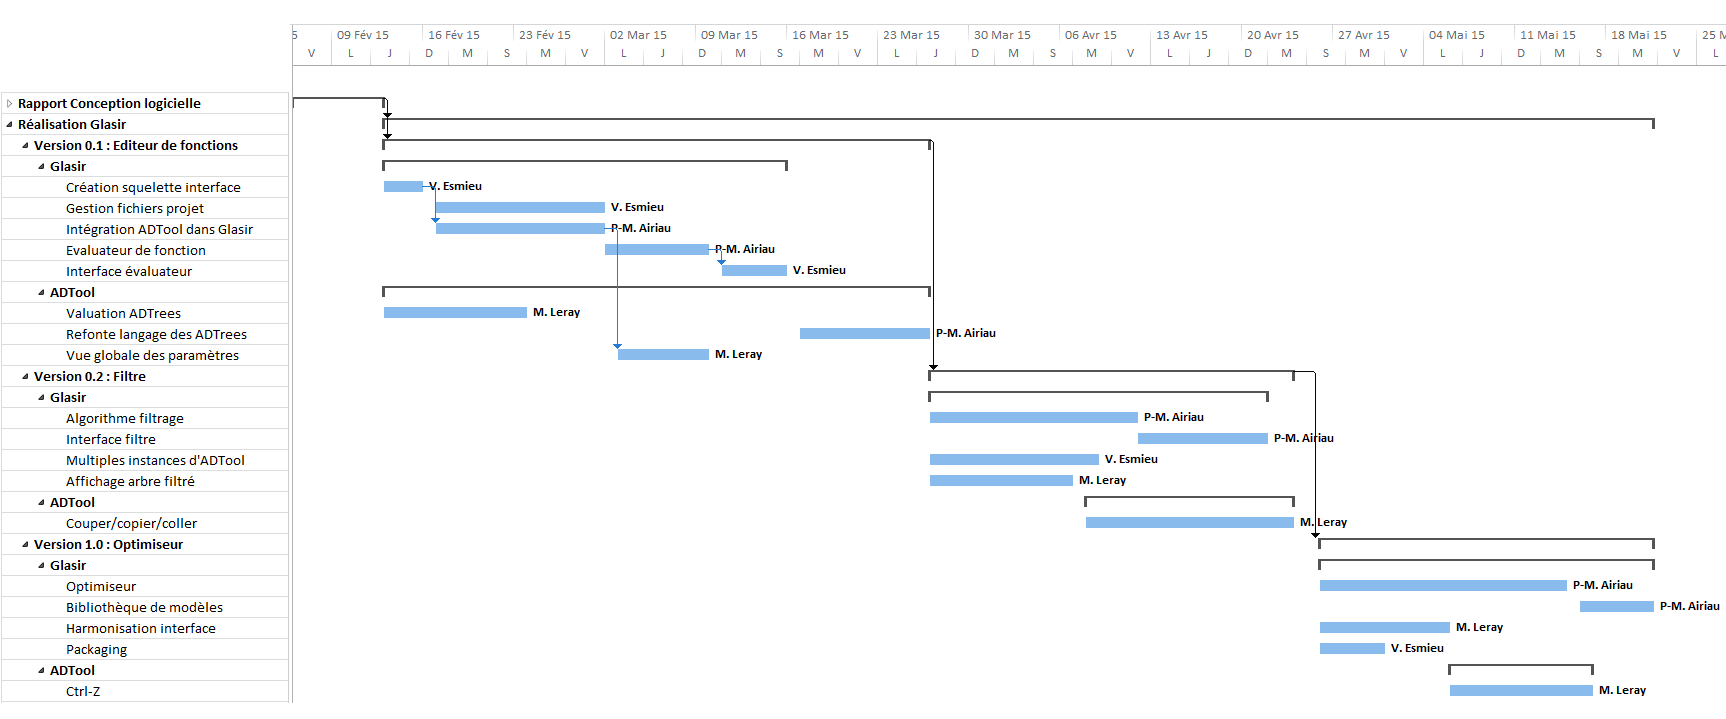
\includegraphics[height=0.70\textwidth]{figure/DiagGantt.png}
	            \caption{Diagramme de Gantt présentant la chronologie des tâches.}
	            \label{fig:gantt}
	        \end{figure}
	    \end{landscape}

		\begin{landscape}
		 	\begin{figure}
	            \centering
	            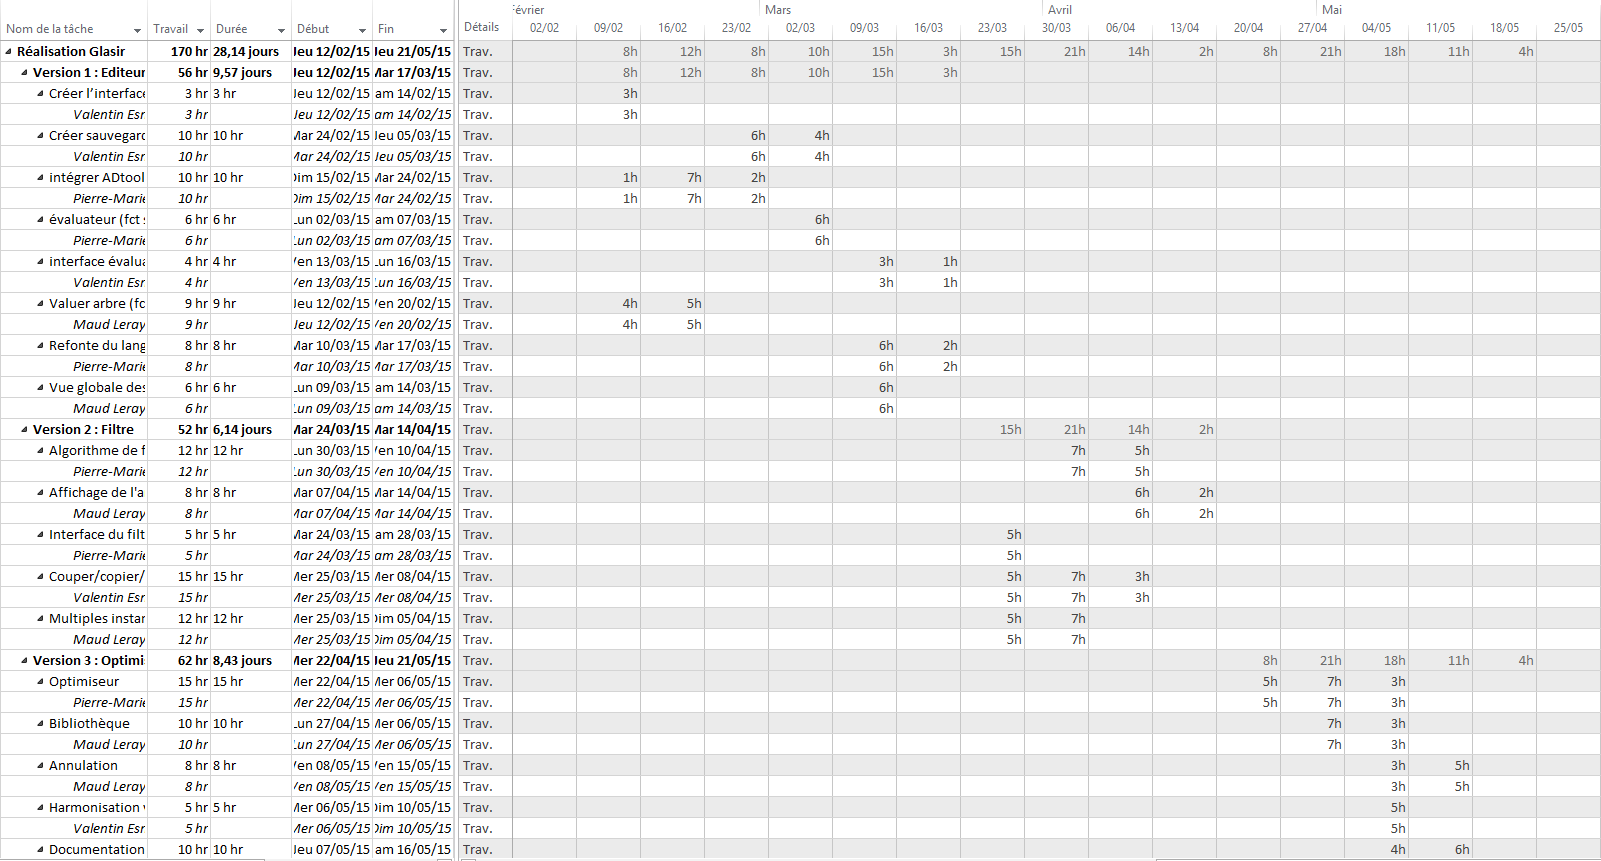
\includegraphics[height=0.70\textwidth]{figure/RepartitionTaches2.png}
	            \caption{Planning des charges réparties par personne}
	            \label{fig:planning_charge}
	        \end{figure}
	    \end{landscape}

	    \subsection{Utilisation des ressources}

    \section{Conclusion}

    %\bibliographystyle{plain}
    %\bibliography{input/biblio}

    % Manoucherie incoming
    \pagevierge
    \ifthenelse{\isodd{\thepage}}
    {\pagevierge}
    {}
    
\includepdf[pages=2]{figure/couv.pdf}
\end{document}